\begin{scriptsize}
•
\end{scriptsize}\documentclass[a4paper,12pt]{report}
 
% Différentes options pour la classe :
% - taille de la fonte    : 10pt, 11pt, 12pt
% - recto ou recto-verso    : oneside, twoside
% - stade de développement    : draft, final
 
% Chargement d'extensions
\usepackage[latin1,utf8]{inputenc}    % Pour utiliser les lettres accentuées
\usepackage[francais]{babel}    % Pour la langue française
\usepackage{graphicx}
 
% Informations le titre, le(s) auteur(s), la date
\title{Rapport de projet : Etrange}
\author {Caroline Keramsi, Florian Thorey, Samuel Mokrani}
\date{\today}
 
% Début du document
\begin{document}
 
\maketitle
\tableofcontents    % Table des matières
\listoffigures        % Liste des figures
 
    \chapter*{Introduction}
    \addcontentsline{toc}{chapter}{Introduction}
    
    \subsection*{Généralités}
    
{Dans le cadre du cours de System On Chips à Télécom Paristech, nous avons du réaliser
un module de traitement vidéo. Plus précisément, ce module devait être capable à partir d'un flux vidéo d'entrée dont les intensités des pixels sont représentées en 256 niveaux de gris, donc codés sur 8 bits, d'établir une transformation géométrique d'ordre 3. Voici les images que nous pouvons obtenir suite à une telle transformation :}
 
\begin{figure}[!h]
	\centering
	\includegraphics[scale = 0.5]{bogart.png}
	\caption{Image non transformée}
\end{figure}

\begin{figure}[!h]
	\centering
	\includegraphics[scale = 0.5]{bogart_tr.png}
	\caption{Image transformée}
\end{figure}

\newpage

	\subsection*{Le backward wrapping}
	
{Afin d'implémenter les transformations géométrique d'ordre 3 à appliquer au flux vidéo transitant par le module Etrange, la technique dite du "backward wrapping" est utilisée. Cette technique est très simple. Elle consiste à calculer, pour chaque pixel de coordonnées (X,Y) de l'image transformée les coordonnées (x,y) de son antécédent dans l'image d'origine.
{
\newline
\newline
$
y = b_{30}X³ + b_{21}X²Y + b_{12}XY² + b_{30}Y³

  + b_{20}X² + b_{11}XY  + b_{02}Y²
  
  + b_{10}X  + b_{01}Y
  
  + b_{00}
$
\newline
$
x = a_{30}X³ + a_{21}X²Y + a_{12}XY² + a_{30}Y³

  + a_{20}X² + a_{11}XY  + a_{02}Y²
 
  + a_{10}X  + a_{01}Y
  
  + a_{00}
$
}
\newline

{Dans ces formules, les $a_{ij}$ et $b_{ij}$ sont des coefficients réels, positifs ou négatifs. Ce qui implique que les coordonnées (x,y) de l'antécédent dans l'image d'origine sont réels, positifs, négatifs aussi. Il s'agit d'un pixel fictif.
Il est donc nécessaire de procéder à une deuxième étape dite d'interpolation afin de calculer l'intensité lumineuse que prendra le pixel de coordonnées (X,Y) dans l'image transformée. Pour cela, on utilise les intensités lumineuses des quatre pixel les plus proches ainsi que les parties entières et décimales des coordonnées (x,y) du pixel antécédent. Ce qui nous donne la formule :
\newline
$$
I = (1-dx).(1-dy).I_{00} + (1-dx).dy.I_{01} + dx.(1-dy).I_{10} + dx.dy.I_{11}
$$
\newline
Où les dx, dy représentent respectivement les parties décimales de x et y et où les $I_{ij}$ représentent les intensités des 4 pixels voisins. Comme toute interpolation elle altère l'image mais nous jugeons que la qualité résultante est acceptable.
\newline
\newline
}
	\subsection*{Quelques précisions}
{



}



	\begin{itemize}
\item Le calcul incrémental : En supposant connu les coordonnées (x,y) de l'antécédent d'un pixel de coordonnées (X,Y), il est possible de calculer, en se basant sur les coordonnées de ce dernier pixel, le pixel antécédent de celui de coordonnées (X+1,Y) et ainsi de suite. 
\item l'interpolation : Comme les coordonnées (x,y) du pixel antécédent ne sont pas forcément entières après le calcul incrémental, il est donc nécessaire de mettre en place une interpolation pour calculer l'intensité du pixel résultant. Cette intensité est obtenue en moyennant les valeurs des intensités des 4 pixels voisins du pixel traité. 
\end{itemize}

	\part*{Architecture retenue}
	\section{Architecture retenue}
	\addcontentsline{toc}{section}{Architecture retenue}
{Pour réaliser ce module de traîtement vidéo, nous avons décidé d'utiliser l'architecture suivante :
 
\begin{figure}[!h]
	\centering
	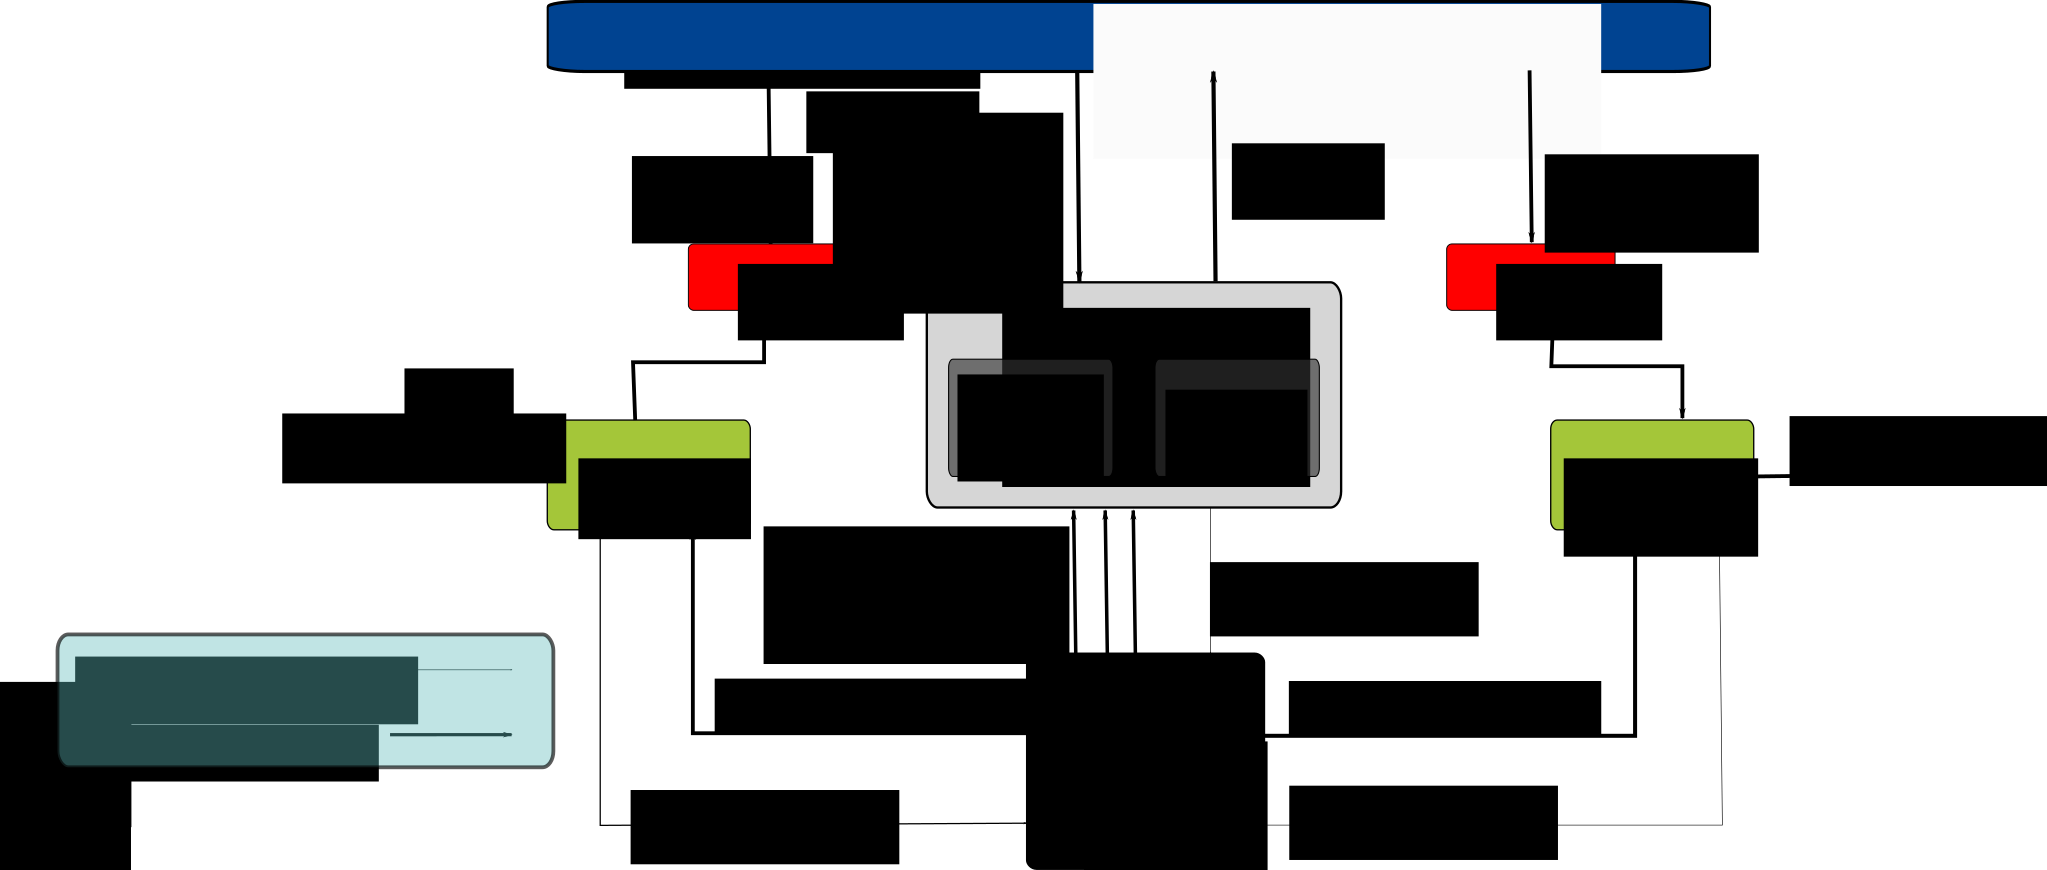
\includegraphics[scale = 0.1]{hardware-arch.png}
	\caption{Architecture}
\end{figure}

Le module VidéoIn se charge de mettre le flux entrant en RAM. VidéoCalc se charge d'aller lire en RAM une image à traîter et à mettre à un autre endroit de la RAM l'image traîtée. Enfin, le module VidéoOut se charge d'aller lire l'image traîtée et de générer un nouveau flux vidéo. Tous ces modules seront pilotés par le processeur (LM32) par le biais d'interruptions. Il enverra aux différents modules les bonnes adresses pour aller lire et écrire en RAM.


Cette architecture a l'avantage d'être modulaire. Par exemple, on peut ne pas utiliser le module de transformation juste en changeant le programme tournant sur le processeur.
}





    \part{Wb\_Slave / VidéoIn / VidéoOut}
    \section{Wb\_Slave}


    \section{VidéoIn}
    \addcontentsline{toc}{section}{VidéoIn}

\begin{figure}[!h]
	\centering
	\includegraphics[scale = 0.5]{video_in.png}
	\caption{Architecture de VidéoIn}
\end{figure}

Le rôle du module VidéoIn est de lire le flux vidéo entrant puis de stocker les images correspondantes en RAM à l'adresse spécifiée par le processeur.
VidéoIn est constitué de deux sous-modules qui correspondent à ces deux fonctions et qui permettent de les exécuter en parallèle. 


\subsection{Module read}
Ce module prend en entrée le flux vidéo constitué du pixel à lire sur 8 bits et des signaux de synchronisation line\_valid et frame\_valid.
Lorsqu'il a détecté un pixel valide, il le place dans une fifo pour le mettre à disposition du module store.\\
La synchronisation entre le module read et le module store est un point délicat. 
En effet la fifo contient uniquement des pixels et ne transportent aucune information concernant leur position dans l'image. 

\paragraph{SystemC}
En systemC, read est implémenté à l'aide d'un SC\_THREAD. 
Il peut ainsi disposer de ses propres compteurs qui lui permettent de se souvenir de la position
du pixel courant dans le flux vidéo.
Il peut ainsi détecter une incohérence sur le flux entrant (trop de pixels sur une ligne par exemple).\\ 
La synchronisation avec store se fait à l'aide d'une variable de classe, first\_address. 
Lorsque store a reçu sa première adresse, il passe ce booléen à vrai.
Le thread read sait alors qu'il pourra commencer à stocker le flux entrant dans la fifo à partir du début de la prochaine image.\\
La fifo est implémenté par une sc\_fifo. 
L'écriture est donc un simple appel à la méthode d'écriture non bloquante nb\_write().
VidéoIn ne peut pas attendre,
si la fifo est pleine au moment de la tentative d'écriture, on sait que l'on ne tient pas le temps réel. 

//TODO changer first\_interrupt en first\_address
//TODO changer le nom des sc\_thread

\paragraph{SystemVerilog}
La fonction read est implémentée en SystemVerilog par le module video\_in\_read qui est instancié dans le module video\_in.
Son implémentation est très semblable au SystemC.\\
On pourra noter une petite difficulté liée à l'utilisation de deux domaines d'horloge différents.
La lecture des pixels entrant se fait sur l'horloge du flux vidéo à 25MHz. 
La fifo, quant à elle fonctionne sur l'horloge système à 100MHz. 
Une écriture dans la fifo se fait par le passage à 1 du signal w\_e. 
Si on générait ce signal dans le bloc séquentiel chargé de la lecture et fonctionnant à 25 MHz,
on risquerait d'écrire 4 fois dans la fifo au lieu d'une.
Pour régler cette difficulté, on génère dans ce bloc un signal write\_fifo\_slow. 
Un autre bloc séquentiel, fonctionnant sur l'horloge système, se charge de générer w\_e lors de la
détection d'un front montant de write\_fifo\_slow.


\subsection{Module store}
Pour commencer, le module store attend que le processeur lui ait fourni une adresse. Pour ce faire il surveille le registre de contrôle du module wb\_slave
qui lui est dédié. Quand celui-ci passe à 1, le module échantillone le contenu du registre d'adresse réservé à VidéoIn. \\
Store rentre ensuite dans la phase de stockage d'une image.
Il attend que NB\_PACK pixels soient présents dans la fifo. Dès que c'est le cas, il les lit et les regroupe par paquets de 4, soit 32 bits,
pour les stocker dans la RAM par une écriture wishbone bloc. 
Lorsqu'il a fini d'écrire une image, le module envoie une interruption au CPU et se met en attente d'une nouvelle adresse.
//TODO à vérifier, peut-être à implémenter
//TODO Mettre les mêmes noms de constantes et les mêmes valeurs entre systemC et systemVerilog//


\paragraph{SystemC}
Store est implémenté en SystemC par un SC\_THREAD.
Ceci permet de se souvenir de l'état précédent du module. 
On peut donc décrire le comportement de store de façon séquentielle.
Le fait de rester dans un état jusqu'à un certain événement est matérialisé par une boucle while contenant un ou plusieurs appels à wait(). \\
La lecture dans la fifo est simple et se fait à l'aide de la méthode read() appliquée à la sc\_fifo.
//TODO compléter sur le fait que la simu n'est pas parfaite car 4 lectures fifo en un temps, où mettre des wait() pour faire une modélisation correcte.

\paragraph{SystemVerilog}
En SystemVerilog, il est nécessaire de changer complètement de paradigme. 
On ne peux pas attendre un événement à l'aide d'une boucle while, 
cela ne serait pas synthétisable! 
Pour décrire un comportement similaire à celui réalisé en SystemC, on a donc mis en place une machine à états.




{}

\newpage
 
    \section*{VidéoOut}
    \addcontentsline{toc}{section}{VidéoOut}

\begin{figure}[!h]
	\centering
	\includegraphics[scale = 0.5]{video_out.png}
	\caption{Architecture de VidéoOut}
\end{figure}

Le fonctionnement de VidéoOut est exactement inverse à celui de VidéoIn.
Il va chercher une image en RAM à une adresse indiquée par le processeur
et génère le flux vidéo correspondant. 
Ces deux fonctions sont effectuées en parallèle par les deux sous-modules de VidéoOut qui se passent
les pixels par une fifo.

\subsection{Le module read}
Ce module va chercher les images en RAM et pose les pixels dans une fifo. 
Il attend que le processeur lui indique qu'une nouvelle adresse RAM est disponible en passant le registre de contrôle de wb\_slave, dédié à VidéoOut, à 1.
Il échantillonne alors le registre d'adresse de VidéoOut.
Une fois cette adresse obtenue, il va lire en RAM par paquets de NB\_PACK pixels, soit NB\_PACK/4 mots.
À chaque paquet obtenu, les mots de 32 bits, découpés en pixel de 8 bits, sont placés dans la fifo dès qu'il y a de la place dans celle-ci.
Une fois la lecture d'une image terminée, read se met en attente d'une nouvelle adresse.

\paragraph{SystemC}
Le module est implémenté à l'aide d'un SC\_THREAD.
Il effectue des écritures bloquantes sur la fifo. 
Sa vitesse est donc limitée par les lectures en RAM et
par le rythme auquel le SC\_THREAD gen vide la fifo.

\paragraph{SystemVerilog}
La problématique est la même que pour le module store de VidéoIn. 
Le style d'écriture en SystemC ne peut pas être reproduit en SystemVerilog.
Le SC\_THREAD a donc été traduit sous la forme d'une machine à états dans le module video\_out\_read instancié par le module video\_out.

\subsection{le module gen}
Gen récupère les pixels qui ont été posés dans la fifo par le module read.
Il génère ensuite le flux vidéo correspondant.

\paragraph{SystemC}
Le code systemC est essentiellement une reprise de video\_gen.
On réalise une lecture non bloquante de la fifo. 
Si la fifo est vide, on le détecte. 
On en déduit que l'on ne tient pas le temps réel.

\paragraph{SystemVerilog}
Le module est implémenté à l'aide d'une machine à états.
Celle-ci fonctionne avec l'horloge du flux vidéo, à 25 MHz.
La lecture dans la fifo, qui fonctionne à 100 MHz doit donc se faire
par l'intermédiaire d'un bloc séquentiel utilisant l'horloge système.
Celui-ci génère le signal r\_ack lorsqu'elle détecte le front montant
du signal r\_ack\_slow contrôlé à 25 MHz.






    \part{Vidéo\_Calc} 
    \section*{Vidéo\_Calc}
    \addcontentsline{toc}{section}{Vidéo\_Calc}
    
    \subsection{Principe}
{La transformation géométrique à appliquer au flux vidéo transitant par le module Etrange doit pouvoir être effectuée en temps réel, c'est à dire que tous les 1/60 de secondes il faut qu'une nouvelle image puisse sortir du module. Le traitement par le processeur de la transformation d'ordre 3 par la technique du backward wraping  à appliquer à l'image ne permet pas de tenir de tels timings. C'est pourquoi un coprocesseur est ajouté au module. Ce coprocesseur que nous avons désigné sous le terme vidéo\_calc est chargé d'implémenter cette technique du backward wraping qui est présentée de manière détaillée dans l'introduction.



}   	
    	Le module Vidéo\_Calc est le module chpaargé d'effectuer la transformation géométrique d'ordre 3 sutr le flux vidéo. Ce traitement doit pouvoir être effectué en temps réel, ce qui implique des contraintes de timing importantes. C'es

{}










    \part{Soft (LM32)} 

    \section*{Soft (LM32)}
    \addcontentsline{toc}{section}{Soft (LM32)}


		\subsection*{Les interruptions}
    \addcontentsline{toc}{subsection}{Les interruptions}
{Le processeur a la charge d'indiquer aux différents modules les adresses à aller lire et écrire les images. Plus précisément :

\begin{itemize}
	\item à Video\_In : envoie de l'adresse où l'image entrante sera stockée
	\item à Video\_Calc : \begin{itemize}
								\item envoie de l'adresse où sera lue l'image à traitée
								\item envoie de l'adresse où sera stockée l'image traîtée
								\item envoie de l'adresse du début des coefficients pour le calcul incrémental
							\end{itemize}
	\item à Video\_Out : envoie de l'adresse où sera lue l'image traîtée
\end{itemize}

Toutes ces adresses sont envoyées suites à des interruptions.
Il y a donc trois principaux handlers d'interruptions : Video\_In\_Handler, Video\_Out\_Handler et Video\_Calc\_Handler.

Le processeur reçoit une interruption de Video\_In lorsque ce dernier a terminé de stocker une image en RAM. Le processeur lui envoit donc une nouvelle adresse pour stocker l'image suivante. Lors de cette interruption, il envoit aussi una adresse de lecture et de stockage à Video\_Calc.
Le processeur reçoit une interruption de Video\_Calc lorsque ce module a terminé de traîter une image. Si l'image traîtée était la première, l'adresse de lecture de l'image traîtée est envoyée à Video\_Out.
Le processeur reçoit une interruption de Video\_Out lorsque ce dernier a terminé de lire une image traitée en RAM. À ce moment là, il envoie une nouvelle adresse à Video\_Out.

Cet enchaînement fonctionne bien en SystemC car le module Video\_Calc est plus rapide que Video\_In et Video\_Out.

//TODO: expliquer les pb que l'on a en Verilog
}
			\subsection*{Gestion de la RAM}
    		\addcontentsline{toc}{subsection}{Gestion de la RAM}
{
	Pour stocker toutes ces images en RAM, on utilise un premier espace contenant les images stockées par Video\_In et un deuxième pour les images stockées par Video\_Calc. Nous pouvons illustrer l'état de la RAM par ce schéma :

\begin{figure}[!h]
	\centering
	\includegraphics[scale = 0.3]{ram_management.png}
	\caption{État de la RAM}
\end{figure}

}

			\subsection*{Initialisation des coefficients pour le calcul incrémental}
    		\addcontentsline{toc}{subsection}{Initialisation des coefficients pour le calcul incrémental}

{La seconde fonctionnalité du processeur est de calculer tous les coefficients nécessaires au calcul incrémental fait par le module Video\_Calc. Pour ceci, nous avons utilisé la représentation en virgule fixe pour que Video\_Calc puisse les récupérer en RAM et faire des calculs avec. Nous utilisons 16 bits pour représenter la partie entière et 16 bits pour la partie fractionnaire. Il y a plusieurs avantages à utiliser la représentation en virgule fixe. La première est que nous connaissons parfaitement la signification de chaque bits du nombre. La seconde est la rapidité des calculs comparé à l'utilisation de flottants.


Pour que le module Video\_Calc puisse récupérer les coefficients en RAM calculé par le processeur, ce dernier lui envoit l'adresse de début de ces coefficients lorsqu'il envoit les adresses de lecture et d'écriture d'images dans Video\_Calc\_Handler.
}

			\subsection*{Calculs pour le chargement du cache}
    		\addcontentsline{toc}{subsection}{Calculs pour le chargement du cache}
{La dernière fonctionnalité du processeur est de calculer les quatre antécédents de chaque tuile et d'en déduire les coordonnées du pixel en haut à gauche du rectangle circonscrit à la partie de l'image qui représente l'antécédent de la tuile en question.
Cette information est envoyée en même temps que les coefficients pour le calcul incrémental.

Ce calcul ne nous permet pas de gérer toutes les transformations possibles : ici, la première transformation se déroulera bien mais la deuxième échouera.
\begin{figure}[!h]
	\centering
	\includegraphics[scale = 0.3]{cache_proc.png}
	\caption{Chargement du cache}
\end{figure}

}



 
    \chapter*{Conclusion}
    \addcontentsline{toc}{chapter}{Conclusion}
{ L'architecture décrite ci-dessus a été implémentée en SystemC dans un premier temps et nous avons arrivons à faire des transformations dans la limite du cache.

//TODO mettre une photo d'une transfo

La traduction en System Verilog n'est pas terminée. Vidéo\_In et Video\_Out sont fonctionnels en System Verilog mais Video\_Calc n'a pas été traduit.

Perspectives et améliorations : 

\begin{itemize}
	\item Traduction de Video\_Calc en System Verilog
	\item	Meilleure gestion du cache pour supporter des transformations plus complexes
	\item Améliorer la partie interpolation car pour l'instant, elle prend 4 cycles
	\item Avoir des coefficients différents pour chaque tuile
	\item La capacité de changer les coefficients pour le calcul incrémental par le clavier 
\end{itemize}
}




% Fin du document
\end{document}
